% Source: graduate-coursework/Prior_Semesters/Fa25/EMCH501/HW2/HW2.tex

\documentclass[border=4pt]{standalone}
\usepackage{amsmath}
\usepackage{amssymb}
\usepackage{graphicx}
\usepackage{tikz}
\usepackage{xcolor}
\usetikzlibrary{shapes.geometric, arrows.meta, positioning, decorations.pathmorphing, patterns}

\begin{document}
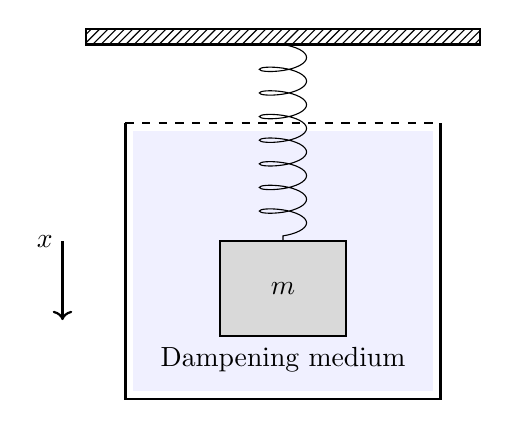
\begin{tikzpicture}[scale=1.0]
  % container with medium
  \draw[thick] (-2,0) -- (-2,-3.5) -- (2,-3.5) -- (2,0);
  \draw[thick,dashed] (-2,0) -- (2,0);
  % medium shading
  \fill[blue!20,opacity=0.3] (-1.9,-0.1) rectangle (1.9,-3.4);
  % dampening medium text
  \node[] at (0,-3) {Dampening medium};
  % ceiling
  \draw[thick,pattern=north east lines] (-2.5,1) rectangle (2.5,1.2);
  \draw[thick] (-2.5,1) -- (2.5,1);
  % spring
  \draw[decoration={coil,aspect=0.3,segment length=3mm,amplitude=3mm},decorate] (0,1) -- (0,-1.5);
  % mass
  \draw[fill=gray!30,thick] (-0.8,-1.5) rectangle (0.8,-2.7);
  \node at (0,-2.1) {$m$};
  % coordinate system
  \node[left] at (-2.8,-1.5) {$x$};
  \draw[->,thick] (-2.8,-1.5) -- (-2.8,-2.5);
\end{tikzpicture}
\end{document}
